%%
%% This is file `sample-nime-paper.tex',
%% generated with the docstrip utility.
%%
%% The original source files were:
%%
%% samples.dtx  (with options: `all,proceedings,bibtex,sigconf')
%% 
%% IMPORTANT NOTICE:
%% 
%% For the copyright see the source file.
%% 
%% Any modified versions of this file must be renamed
%% with new filenames distinct from sample-nime-paper.tex.
%% 
%% For distribution of the original source see the terms
%% for copying and modification in the file samples.dtx.
%% 
%% This generated file may be distributed as long as the
%% original source files, as listed above, are part of the
%% same distribution. (The sources need not necessarily be
%% in the same archive or directory.)
%%
%%
%% Commands for TeXCount
%TC:macro \cite [option:text,text]
%TC:macro \citep [option:text,text]
%TC:macro \citet [option:text,text]
%TC:envir table 0 1
%TC:envir table* 0 1
%TC:envir tabular [ignore] word
%TC:envir displaymath 0 word
%TC:envir math 0 word
%TC:envir comment 0 0
%%
%%
%% History of NIME Template Updaters:
%% Modified by Anna Xambó Sedó, Benedict Gaster, João Tragtenberg, 31 October 2025
%% Modified by Florent Berthaut, Charles Martin, Yichen Wang, 21 November 2024
%% Modified by Adnan Marquez-Borbon 30 November 2022
%% Modified by Courtney Reed 28 November 2022
%% Modified by Joe Wright 14 December 2019
%% Modified by Niccolò Granieri 10 October 2018
%% Modified by Angelo Fraietta 23 December 2018
%% Modified by Angelo Fraietta 22 November 2018
%% Modified by Rodrigo Schramm on 22 September 2018
%% Modified by Luke Dahl on 17 October 2-17
%% Modified by Cumhur Erkut on <2016-10-11 Tue>
%% Modified by Edgar Berdahl on 5 November 2014
%% Modified by Baptiste Caramiaux on 25 November 2013
%% Modified by Kyogu Lee on 7 October 2012
%% Modified by Georg Essl on 7 November 2011
%%
%% And here's the template:
%%
%% The first command in your LaTeX source must be the \documentclass
%% command.
%%
%% For submission and review of your manuscript please change the
%% command to \documentclass[sigconf, anonymous, review]{nimeart}.
%%
%% When submitting camera ready, please change the command
%% to \documentclass[sigconf]{nimeart}
%%
% \documentclass[sigconf,anonymous,review]{nimeart}
\documentclass[sigconf]{nimeart}
%%

%% This package avoids urls margin overflow
\usepackage{xurl}

\usepackage{CJKutf8}

%% \BibTeX command to typeset BibTeX logo in the docs
\AtBeginDocument{%
  \providecommand\BibTeX{{%
    Bib\TeX}}}

\setcopyright{cc}
\copyrightyear{2026}
\acmYear{2026}
\acmDOI{}

%% These commands are for a PROCEEDINGS abstract or paper.
%% Make sure this is up to date with the correct edition of NIME.
\acmConference[NIME '27]{International Conference on New Interfaces for Musical Expression}{June 23--26,
  2027}{Paris, FR}
%% This suppresses the ACM Reference Format printing.
\settopmatter{printacmref=false}
\acmISBN{}

%%
%% end of the preamble, start of the body of the document source.
\begin{document}

%%
%% The "title" command has an optional parameter,
%% allowing the author to define a "short title" to be used in page headers.
\title {UWBs in Interactive Installations}


%% The "author" command and its associated commands are used to define
%% the authors and their affiliations.
%% Of note is the shared affiliation of the first two authors, and the
%% "authornote" and "authornotemark" commands
%% used to denote shared contribution to the research.
\author{Alejandro Suarez}

\email{asuarez43@gatech.edu}
\affiliation{%
  \institution{Georgia Institute of Technology}
  \city{Atlanta}
  \state{GA}
  \country{United States}
}

\author{Orlando Kenny}

\email{orlando@meatatlanta.org}
\affiliation{%
  \institution{M.E.A.T.}
  \city{Atlanta}
  \state{GA}
  \country{United States}
}

\author{Matias Cevallos}

\email{mats@meatatlanta.org}
\affiliation{%
  \institution{M.E.A.T.}
  \city{Atlanta}
  \state{GA}
  \country{United States}
}

\author{Mia Wood}

\email{orlando@meatatlanta.org}
\affiliation{%
  \institution{Georgia Institute of Technology}
  \city{Atlanta}
  \state{GA}
  \country{United States}
}

\author{Henrik non Coler}
\email{hvc@gatech.edu}
\affiliation{%
  \institution{Georgia Institure of Technology}
  \city{Atlanta}
  \state{GA}
  \country{United States}
}


%% ATTENTION: CHANGE THE LINE BELOW
%% Shortened Authors' Names:
\renewcommand{\shortauthors}{First Author's Surname et al.}
%% By default, the full list of authors will be used in the page
%% headers. Often, this list is too long, and will overlap
%% other information printed in the page headers. This command allows
%% the author to define a more concise list
%% of authors' names for this purpose.

%%
%% The abstract is a short summary of the work to be presented in the
%% article.
\begin{abstract}

 Within the ever expanding continuum of immersive sound and media installations, artists continually seek new technologies to expand their creative toolkits'. One technology that has remained underutilized in this immersive movement is Ultra-Wideband (UWB) sensing. This paper investigates the successful implementation of UWB sensors housed in custom wearables used for sound manipulation in a communal musical instrument, examining the technology's strengths and limitations while exploring potential future applications for UWB-powered musical interaction.....

 In this installation users are able to explore a projection mapped virtual environment that reacts to their standing position. This environment is rendered in Unreal engine and is projected on the floor. Encompassing the projection mapped are are 4 speakers playing a global soundscape, and on each UWB wearable there is a speaker which created a local soundscape for each user. .....

\end{abstract}

%%
%% Keywords. The author(s) should pick words that accurately describe
%% the work being presented. Separate the keywords with commas.
\keywords{Ultra-Wideband, Wearables, Super Collider, Touch Designer, Unreal Engine}
  
%% A "teaser" image appears between the author and affiliation
%% information and the body of the document, and typically spans the
%% page. Suggested dimensions: 1200x400px
\begin{teaserfigure}
  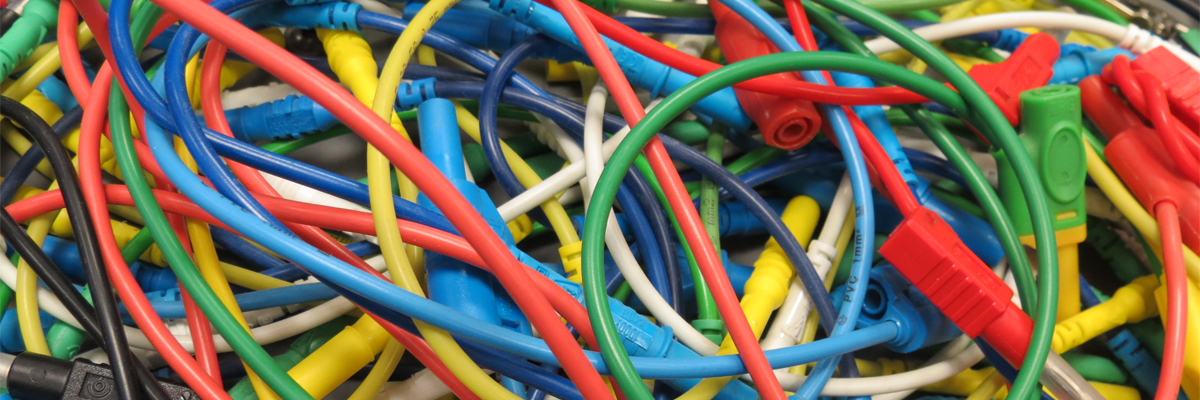
\includegraphics[width=\textwidth]{images/sampleteaser.png}
  \caption{Entangled meshwork of colorful banana patch cables. Image by WikiProfPC (CC BY-SA 4.0)}
  \Description{Tangled banana patch cables}
  \label{fig:teaser}
\end{teaserfigure}

%%
%% This command processes the author and affiliation and title
%% information and builds the first part of the formatted document.
\maketitle

\section{Introduction}

Since the dawn of time, humans have been immersed and interacted with. 

\section{Related Work}

While this project utilized UWBs in this specific way, here are some related projects that utilized UWBs to achieve similar goals.. 

\section{Technologies}

This project uses a modular platform architecture that relies on a central python script to provide a continuous stream of data. This data is packaged as a JSON string and distributed over OSC to the rest of the software over a local network. 

\subsection{Project Architecture}
The project architecture consists of... 

UWB -> Python -> Super Collider -> Wearable and Speakers
              
      
UWB -> Python -> Unreal Engine -> Touch Designer -> Projectors


\subsection{UWBs}

UWB anchors are placed on 4 corners of the virtual environment and focus on triangulating the position of the active wearable when they enter.... 

\subsection{Super Collider}

\subsection{Unreal Engine}

\subsection{Touch Designer}

\section{Wearable}

\subsection{Industrial Design}

\subsection{Embedded Electronics}

\subsection{Fabrication}




\section{Activity Report}

This installation was presented over a two week period at a gallery at The Georgia Institute of technology where we demonstrated two different methods of interaction with the UWB wearables.  During week 1 the position of the wearable in relation to the virtual environment affected the sounds they outputted. During week 2 the relative position between each UWB wearable changed the sound they outputted, encouraging users to get closer or further form one another to manipulate their local soundscape... To track the effectiveness and enjoyment of these levels of feedback we had users submit answer a short questionnaire and found that they preferred.... (not sure if the questionnaire we had guests fill out is admissible without IRB certification?) 



\section{Conclusion}

This paper presented a communal instrument that utilizes sound reactive UWB wearables as the primary means of detecting movement interaction within a virtual environment.... 

We think it is a useful underexplored technology in the immersive installation world that would work well in large rooms and can provide detailed data...

There are real limitations of the UWBs in musical applications including occlusion when line of sight is interrupted between two sensors... etc

\nocite{*}


\bibliographystyle{ACM-Reference-Format}
\bibliography{references}

\end{document}
\endinput
%%
%% End of file `sample-nime-paper.tex'.
